%Author: HU Pili
%Start Date: Dec 8, 2012
%Template: ACM Sig template. (preamble comments are moved to the end)

\documentclass{sig-alternate}

\usepackage[tight,footnotesize]{subfigure}
\usepackage{url}
%HU, Pili
%Create: 20120330
%Modify: 20120330
%The unified entry to include in my tutorial series

%HU, Pili
%Create: 20110910
%Modify: 20120330
%purpose of this file is to gather commonly used
%mathematical abbreviations, to speed up writing
%notes

%\usepackage[utf8x]{inputenc}
%\usepackage{ucs}
%\usepackage{amsmath}
%\usepackage{amsfonts}
%\usepackage{amssymb}
%\usepackage{amsthm}
\usepackage{url}
\usepackage{graphicx}

%\usepackage{fancyhdr}
%\pagestyle{fancy}
%\fancyhead{}

%=====Calculus======
%the following commands are not originated by me
%I pick them from http://www-solar.mcs.st-and.ac.uk/~clare/Latex/
%the following line controls the style of patial derivative
%1), use \dfrac, height is larger, looks good. 
%2), use \frac, also work, but space looks limited. 
\newcommand{\myfrac}[2]{\dfrac{#1}{#2}}
\newcommand{\diff}[2]{\myfrac{{\rm d}#1}{{\rm d}#2}}
\newcommand{\ndiff}[3]{\myfrac{{\rm d}^{#3}#1}{{\rm d}#2^{#3}}}
\newcommand{\pdiff}[2]{\myfrac{\partial #1}{\partial #2}}
\newcommand{\npdiff}[3]{\myfrac{\partial^{#3} #1}{\partial #2^{#3}}}
\newcommand{\e}[1]{\ensuremath{{\rm e}^{#1}}}
\newcommand{\ldiff}[2]{\ensuremath{{\rm d}#1/{\rm d}#2}}
\newcommand{\lpdiff}[2]{\ensuremath{\partial#1/\partial#2}}
\newcommand{\lnpdiff}[3]{\ensuremath{\partial^{#3}#1/\partial#2^{#3}}}
\newcommand{\dif}[1]{\mathrm{d}#1}

%20120330
%The reason I don't copy the original file as a whole
%is that it contains too many individually preferred 
%definitions. 
%
%I start with those basic symbols and adapt them in use. 

%=====Matrix======
\newcommand{\tr}[1]{\mathrm{Tr}\left[#1\right]}
\newcommand{\tran}[1]{#1^\mathrm{T}}
\newcommand{\her}[1]{#1^\mathrm{*}}
%The following shorthand of matrix may be convenient. 
%However, it is so short that I'm worried it may 
%collide with something else. I don't use at present.
%\newcommand{\m}[1]{\mathbf{#1}}
\newcommand{\adj}[0]{\mathrm{adj}}
\newcommand{\inv}[1]{#1^{-1}}


%=====Theorem definitions=====
%\newcounter{mytheoremorder}
%\newtheorem{mydef}{Definition}
%\newtheorem{myaxm}{Axiom}
%\newtheorem{mylm}{Lemma}
%\newtheorem{mythm}[mytheoremorder]{Theorem}
%\newtheorem{myprop}[mytheoremorder]{Proposition}
%\newtheorem{myex}{Example}

%=====Optimization====
\DeclareMathOperator*{\argmax}{arg\,max}
\DeclareMathOperator*{\argmin}{arg\,min}
\DeclareMathOperator*{\minimize}{minimize}
\DeclareMathOperator*{\maximize}{maximize}
%\newcommand{\maximize}[0]{\mathrm{Maximize~}}
%\newcommand{\minimize}[0]{\mathrm{Minimize~}}

%=====Probability====
\newcommand{\E}[0]{\mathbb{E}}
\newcommand{\var}[0]{\mathrm{Var}}
\newcommand{\cov}[0]{\mathrm{Cov}}

%=====Quick and Unified Reference====
%20120505
%Usage: \eq{\ref{xxx}}
%The reason I keep "\ref" away from definition, 
%and let user type it every time is that: 
%currently I'm working on Texmaker, and it can 
%trigger a selection panel when the sequence 
%"\ref" is found. Maybe further configuration of 
%texmake can make it do the same thing when the 
%following self-defined sequence is detected.
%This is left for future work. 
\newcommand{\req}[1]{\textbf{Eq~{#1}}}
\newcommand{\rfig}[1]{\textbf{Fig~{#1}}}
\newcommand{\rtbl}[1]{\textbf{Tbl~{#1}}}
\newcommand{\rpg}[1]{\textbf{P~{#1}}}
\newcommand{\rsec}[1]{\textbf{Section~{#1}}}
\newcommand{\ralg}[1]{\textbf{Alg~{#1}}}



%algorithm
\usepackage{algorithmic}
\usepackage{algorithm}
\floatname{algorithm}{Algorithm}
\renewcommand{\algorithmicrequire}{\textbf{Input:}}
\renewcommand{\algorithmicensure}{\textbf{Output:}}

\usepackage{glossaries}
\newacronym{sns}{SNS}{Social Networking Services}
\newacronym{osn}{OSN}{Online Social Networks}
\newacronym{dsn}{DSN}{Decentralized Social Network}
\newacronym{msn}{MSN}{Mobile Social Network}
\newacronym{dtn}{DTN}{Delay Tolerant Network}
\newacronym{nfc}{NFC}{Near-Field Communication}
\newacronym{d2d}{D2D}{Device-to-Device}
\newacronym{ppr}{PPR}{Personalized PageRank}
\newacronym{pr}{PR}{PageRank}
\newacronym{xmpp}{XMPP}{Extensible Messaging and Presence Protocol}
\newacronym{roc}{ROC}{Receiver Operating Characteristics}
%\newacronym{roca}{ROCA}{Receiver Operating Characteristics Area}
%\newacronym{auc}{AUC}{Area Under the (ROC) Curve}
\newacronym{auc}{AUC}{Area Under the ROC Curve}
\newacronym{tpr}{TPR}{True Positive Rate}
\newacronym{fpr}{FPR}{False Positive Rate}
\newacronym{ev}{EV}{Escape Vector}
\newacronym{rw}{RW}{Random Walker}
\newacronym{srfe}{SRFE}{SNSRouter Front End}

\begin{document}
\conferenceinfo{
	Please ignore the above and following Copyright statements. 
	It's from the template. 
}{...}

\title{ {\ttlit SNSRouter} -- 
	A Framework for  \\
	Intelligent Message Routing on Heterogeneous SNS
	\titlenote{
		Source codes of the paper and project can be found 
		in the following Github repository. 
		This repository is continuously evolving. 
		\url{https://github.com/hupili/sns-router}
	}
}
%\subtitle{
%	Middleware for SNS's and Flexible Personalized Ranking Framework
%}
%\subtitle{[Extended Abstract]
%}}

%
% You need the command \numberofauthors to handle the 'placement
% and alignment' of the authors beneath the title.
%
% For aesthetic reasons, we recommend 'three authors at a time'
% i.e. three 'name/affiliation blocks' be placed beneath the title.
%
% NOTE: You are NOT restricted in how many 'rows' of
% "name/affiliations" may appear. We just ask that you restrict
% the number of 'columns' to three.
%
% Because of the available 'opening page real-estate'
% we ask you to refrain from putting more than six authors
% (two rows with three columns) beneath the article title.
% More than six makes the first-page appear very cluttered indeed.
%
% Use the \alignauthor commands to handle the names
% and affiliations for an 'aesthetic maximum' of six authors.
% Add names, affiliations, addresses for
% the seventh etc. author(s) as the argument for the
% \additionalauthors command.
% These 'additional authors' will be output/set for you
% without further effort on your part as the last section in
% the body of your article BEFORE References or any Appendices.

\numberofauthors{1} %  in this sample file, there are a *total*
% of EIGHT authors. SIX appear on the 'first-page' (for formatting
% reasons) and the remaining two appear in the \additionalauthors section.
%
\author{
% You can go ahead and credit any number of authors here,
% e.g. one 'row of three' or two rows (consisting of one row of three
% and a second row of one, two or three).
%
% The command \alignauthor (no curly braces needed) should
% precede each author name, affiliation/snail-mail address and
% e-mail address. Additionally, tag each line of
% affiliation/address with \affaddr, and tag the
% e-mail address with \email.
%
% 1st. author
\alignauthor
    Pili Hu
    \titlenote{\url{http://personal.ie.cuhk.edu.hk/~hpl011/}} \\
    \affaddr{Information Engineering}\\
    \affaddr{The Chinese University of Hongkong}\\
    \affaddr{Shatin, NT, Hongkong}\\
    \email{hupili@ie.cuhk.edu.hk}
}

\maketitle
\begin{abstract}
	Online Social Networks (OSN) has become an essential part of human life today. 
	They also share a very large portion of Internet traffic in terms of Page Visits. 
	Successful OSNs are like Facebook, Twitter, Renren, SinaWeibo, etc. 
	Two of the basic functions are: 1) maintain connections with people; 
	2) read/write updated information in a networked fashion. 

	In this paper, we focus on the function of \textbf{information acquisition and dissemination}.
	We build a middleware for heterogeneous Social Network Services (SNS), 
	thus enabling very easy cross-platform message manipulation. 
	Besides those traditional OSNs, we can also abstract RSS, Email, SQLite 
	and more other platforms in the same way. 
	With this middleware, SNSAPI \cite{github_snsapi}, 
	many novel applications can be built and they are ready 
	to be extended to other platforms. 

	We observe that message forwarding is a popular operation on SNS
	and there are many manual cross-platform forwarding behaviours. 
	SNSRouter \cite{github_snsrouter} project aims at developing 
	an easier way to perform cross-platform message forwarding (routing). 
	We propose to leverage combined human and machine intelligence. 
	More specifically, we propose a Rank Preserving Regression (RPR) formulation 
	to personalize incoming messages' ordering. 
	Users with certain programming knowledge can easily add other personalization features. 
	An appropriate ordering saves user's time in reviewing those messages. 
	He/she can then make final forwarding decisions efficiently. 

	Evaluation on real traces collected by SNSRouter shows that 
	RPR outputs very good weighting even with elementary feature extractions. 
	The author of the report, who is not an expert in NLP, can construct those features in one day. 
	This shows the flexibility of our system and algorithm framework. 
\end{abstract}

\category{H.3}{INFORMATION STORAGE AND RETRIEVAL}{Systems and Software}
\category{M.5}{KNOWLEDGE PERSONALIZATION AND CUSTOMIZATION}{Framework}

\terms{System, Algorithm}

\keywords{
	Social Network Services, 
	Middleware, 
	Personalization,
	Rank Preserving Regression
}

\section{Introduction}
\label{sec:Introduction}

Social Network Services mimic the real life social networks using modern technology. 
They come in many different forms. 
In this section, we first introduce different Social Network Services
and provide a unified view of them. 
Then we introduce cross-platform message forwarding (routing), 
which motivates the SNSRouter project. 

\subsection{Heterogeneous Social Network Services}
\label{sec:Heterogeneous Social Network Services}

There are many \gls{sns} nowadays.
\rfig{\ref{fig:sns-het}} 
illustrates some of them. 
If we focus on information acquisition and dissemination
in a networked fashion, 
they can all be casted in the same way:
\begin{itemize}
	\item \gls{osn}. Examples are like Facebook, Twitter, 
		Renren, SinaWeibo, TecentWeibo in the figure. 
		People form links (either directed or undirected) first
		and information can flow on those links. 
	\item Communication Networks.  
		Examples are like telephone network, SMS network and Email network. 
		On those network, links do not need to be established beforehand. 
		Sender can specify receiver(s) explicitly on the fly. 
	\item Information Sources. 
		Examples are like RSS feeds of blogs and keywords on search engines. 
		When one subscribe to RSS feeds or write a script to monitor the 
		response of a certain keyword search engine, 
		a unidirectional link is established from the information sources to him/her. 
\end{itemize}

As one can see, the only differences are:
1) whether links are formed beforehand;
2) whether links are directed or undirected;
3) whether read/write are allowed or only read (or write) is allowed;
4) whether user authentication/authorization are required.
Currently, there is no efficient way to abstract all these platforms, 
so we see people visiting several \gls{sns}'s everyday. 

\begin{figure}[t!]
	\centering
	\includegraphics[width=0.9\linewidth]{../pic/sns-het.pdf}
	\caption{Illustration of Heterogeneous SNS}
	\label{fig:sns-het}
\end{figure}

\subsection{Cross Platform Message Forwarding}
\label{sec:Cross Platform Message Forwarding}

Information dissemination in a single domain is natural. 
Many platforms have built-in ``forward'' functions, 
e.g. ``retweet'' on twitter, ``forward'' in email, etc. 
Many researches have also been done for information dissemination on a single platform. 
However, cross-platform behavior is a seldom discussed topic. 
We believe this is largely due to lack of mature engineering models
and large collection of data sets. 
Nevertheless, we observe many manual cross-platform behaviours.
For example:

\begin{itemize}
	\item 
	You subscribe to a blog RSS and read a gossip on it.
	The gossip is interesting so you copy and paste it to Renren. 
	%Renren is an OSN, which is typical SNS in our traditional understanding.
	%Blog, from the subscriber's point of view, is also a kind of SNS, but is read-only.
	\item 
	You receive Google Scholar updates on a certain topic by email.
	Once there are some eye-catching new papers, you forward to your colleagues by email.
	%Email is also SNS, where the link is formed dynamically and message is targeted instead of being posted on a wall.
	\item
	Now iPhone 5 is a big event and you want to get latest news about it.
	Instead of following ``inbridge'' at ``twitter'', you can follow ``iphone+5'' at ``baidu''
	(by automatically poll the link: \url{http://www.baidu.com/s?ie=utf-8&wd=iphone+5}). 
	%Traditionally, you follow some guy on Sina Weibo or Twitter.
	%This guy always keeps an eye on big tech news so you are informed of the latest news.
	%Here's an alternative: \url{http://www.baidu.com/s?ie=utf-8&wd=iphone+5}.
	%You can think of ``baidu'' as an SNS, where there are many people who usually give you the updated messages on a certain topic.
	%Of course, after getting the news, you are very likely to forward it to Sina Weibo.
	%(Congratulations! You stand at the frontier now!!)
\end{itemize}

Note the roles people play in the above examples. 
We know Internet routers connect different IP subnet. 
Analogously, those people are routers across different \gls{sns}s. 
The routing job is done manually at preset. 
How about making it automated or semi-automated? 
Can we learn one's preference and use machine intelligence to assist the routing?  

\subsection{Organization}
\label{sec:Organization}

SNSRouter \cite{github_snsapi} is built on a prior work -- SNSAPI \cite{github_snsapi}.
In order to make this document self-contained, 
we will also include SNSAPI in the system design section. 
%SNSAPI and SNSRouter as a whole. 

In 
\rsec{\ref{sec:Related Work}}
, we briefly survey related work. 
In 
\rsec{\ref{sec:Philosophy}}
, we discuss design philosophy of SNSAPI and SNS-Router. 
In 
\rsec{\ref{sec:System Framework}}
, we present the system framework. 
In 
\rsec{\ref{sec:Formulation}}
, we formulate the personalization problem as Ranking Preserving Regression. 
In
\rsec{\ref{sec:Algorithm Design}}
, we transform the problem and propose to use 
Stochastic Gradient Descent (SGD) as the training algorithm. 
In 
\rsec{\ref{sec:Evaluation}}
we evaluate all aspects of our algorithm framework:
efficiency, accuracy, robustness, and flexibility. 
Last, we conclude this paper in 
\rsec{\ref{sec:Conclusion}}
and share our visions on future works in 
\rsec{\ref{sec:Future Work}}
.

Users who want to get hands on quickly can skip the those 
system and algorithm discussions and 
consult the executive summary in Appendix \ref{sec:Executive Summary of SNSRouter Usage}. 
When time is permitted, we encourage you to come back 
and read those discussions to get a better picture 
so that you can full utilize the power of SNSRouter. 

%    sec:Related Work
%    sec:Philosophy
%    sec:System Framework
%    sec:Formulation
%    sec:Impossibility of Complete Auto Forwarding
%    sec:The Problem of Classification
%    sec:Regression Formulation
%    sec:Algorithm Design
%    sec:Induce Preference Relations on Graph
%    sec:Straight Optimization Solver
%    sec:Problem Transformation
%    sec:Gradient Descent
%    sec:Stochastic Gradient Descent
%    sec:Evaluation
%    sec:HU's Data Set
%    sec:Criterion
%    sec:Efficiency and Complexity
%    sec:Robustness
%    sec:Case Study -- Add ``echo'' Feature
%    sec:Conclusion
%    sec:Future Work

% ==== past paragraphs in proposal ====
%We observe many such cross-domain forwarding behaviors everyday! 
%However, we lack abstraction of those platforms and differently formatted messages. 
%Users don't have a unified way to perform easy forwarding. 
%Researchers don't have cross-domain data for study. 
%We take an initial step towards this direction. 
%The open-source SNSAPI project develops a middle ware to unify different SNS (OSN, RSS, email, etc).
%Different SNSs are abstracted in the form of channel and they support primitives like auth(), read(), write().
%The SNSAPI project is at its infancy.
%We'll spend some time contributing to SNSAPI but do not count it in the SNSRouter project.
%The SNSRouter project lies on SNSAPI (App layer in SNSAPI terminology). 
%We'll focus on prototyping an easy way to route cross-domain messages. 
%On this prototype system, we'll be able to collect trace data. 
%Using this cross-domain routing data, we can train algorithms to intelligently make forwarding decisions.
%We plan to leverage topology (e.g. come from whom), 
%content (e.g. the topic) and context (e.g. time of day / location of user) features.
%It's worth to note that SNSAPI framework enables very flexible usage.
%One can configure an archive channel (e.g. email) 
%and write all messages he like there for future retrieval. 
%In this case, the routing (originally can be multiple-input-multiple output) 
%degrades to a multiple-in-single-out personal recommender system.
%To make things tractable, we'll start with the recommender algorithm using all three kinds of features.

\section{Related Work}
\label{sec:Related Work}

From the system aspect, some Internet resource aggregation services are related. 
From the algorithm aspect, some personalization services are related. 
In this section, we briefly survey those services. 

\subsection{Aggregation Services}
\label{sec:Aggregation Services}

There are many aggregation services on the Internet. 
Some of them focus on dealing with a certain type of sources, 
e.g. Google Reader for RSS feeds. 
Some of them can aggregate heterogeneous sources, 
like ifttt \cite{ifttt} and Yahoo Pipes \cite{yahoo_pipes}. 

ifttt abstracts services on the Internet by ``channel'' 
(we borrow this term in SNSAPI), 
e.g. Facebook, Twitter, RSS, SMS, etc. 
Users can define forwarding rules (called ``recipe'' on ifttt)
in this manner:
IF This happens, Then do That (IFTTT). 
This service is very handy for normal users who simply want to bridge several services, 
e.g. publish status on Facebook and the message is automatically forwarded to Twitter. 
ifttt supports a wide spectrum of platforms, 
but there is little flexibility for user to build advanced rules. 

Yahoo Pipes (YP), on the contrary, supports less platforms but allows somewhat advanced rules. 
YP focus on the traditional web, so operations like 
fetching webpage, RSS feeds and CVS table are supported. 
In the pipe construction UI, users can drag sources 
and logic modules (e.g. condition, loop, etc) to the design board
and connect them using ``pipe''.
In the Web1.0 world, YP could be a good aggregator. 
However in the web2.0 world, 
User Generated Content (UGC) is dominating 
and it is full of noise. 
Simple constructions provided by YP is far from enough. 
e.g. forward a certain topic RSS entries to somewhere else. 

\subsection{Personalization with Machine Intelligence}
\label{sec:Personalization with Machine Intelligence}

One major problem of those \gls{sns}'s is that there are too 
many messages flowing throughout the network. 
Even the data rate within one's personal view is too large for human to process efficiently. 
%The noise level is too high to prevent people from 
%acquiring information efficiently. 
%is significantly lowered. 
%efficiency of 
Besides filtering out noise, one also want to prioritize the display of messages 
so that messages can be processed by human in descending order of their importance. 
Different users have different preference so personalization is needed. 
Towards this end, many service providers also develop their own 
machine learning algorithms to help users personalize the incoming messages. 

Personalized incoming message ranking is of its own research interest 
even in the case of single platform. 
For example, SinaWeibo by default presents incoming messages 
in reverse chronological order. 
Users can enable ranked view and obtain a probably more informative timeline. 
For another example, GMail classifies incoming messages 
into ``important'' and ``ordinary'' types 
so that users can process ``important'' messages first. 

Existing approaches focus more on developing better algorithms. 
Training data is obtained mostly by implicit feedback, 
e.g. how long a user stays on one message. 
User engagement in the training cycle is very low. 
Thus the degree of personalization is also low. 
Besides, those service providers target mass audience
and provide no flexibility for people who understands how to program. 
For example, one may suffer spontaneously from someone's overwhelming messages. 
The common practice is to block his/her messages (not unlink the user). 
However, service providers usually set an upperbound on the number users blocked, 
e.g. 5 for Renren and 15 for SinaWeibo. 
One needs to upgrade his/her account to paid member in order to grow the upperbound. 
Anyone who knows programming agrees that blocking specified users
is a very simple task given proper programming interface. 
To avoid blocking spontaneous noise sources permanently, 
one can also set some timeout logic or probabilistic blocking logic. 
However, all of those simple operations are not possible in current services. 

On one hand, existing personalization approaches try to 
solve harder than necessary problems with little user side knowledge. 
On the other hand, some simple personalization demand 
can not be implemented by the users. 

\section{Philosophy}
\label{sec:Philosophy}

In this section, we discuss the design philosophy 
of our system framework and algorithm framework. 
In a word, we pursue simple but effective approaches
which leverage human and machine intelligence simultaneously. 

\begin{itemize}
	\item \textbf{Focus on solving 80\% problems}. 
		The Pareto Principle \cite{wiki_pareto} tells us that 
		(qualitatively) one only needs 20\% effort to solve 80\% problems; 
		In order to solve the rest 20\% problems, he/she needs to 
		spend the other 80\% time. 
		Example: conceptually, we only abstract three methods for \gls{osn}, 
		namely \textbf{read}, \textbf{write} and \textbf{auth}. 
		The three methods can cover more than 80\% functions one need on an \gls{osn}. 
		They are also universal across many other \gls{sns}. 
		However, in order to abstract many platform specific functions, 
		we need much more time, but those functions may be seldom used 
		in our cross-platform settings. 
	\item \textbf{Keep It Simple and Stupid (KISS)} \cite{wiki_kiss}. 
		Whenever possible, we prefer simpler solutions. 
		Common and hard cut rules will be implemented directly with configurable interface. 
		e.g. one can configure some channels to be read-only and others to be write-only directly. 
		We do not need to ``learn'' such preference through user interaction. 
		%2) When simpler features are effective enough, we do not consider advanced features. 
		%3) When simpler 
		This principle also applies to our algorithm framework design, 
		i.e. When simpler features are effective enough, we do not consider advanced features;
		When linear combination is good enough, we do not bother to look at non-linear combinations. 
	\item \textbf{Combine human and machine intelligence}. 
		In \rsec{\ref{sec:Related Work}} we discussed the current approaches adopted by 
		both industry and research communities. 
		Machine learning algorithms are asked to do much harder tasks than necessary. 
		For one extreme example, one can put all bits of a message 
		(sender, text, time, etc) into one very long vector as feature. 
		If we have a very powerful machine learning algorithm, it may be able to 
		learn what factor is important to personalize one's messages and rank them reasonably. 
		Such algorithm, even exists, will be very costly. 
		However, the user speaks louder than any statistical clues.  
		If one user always prefer longer messages than shorter message, 
		he/she just put the length of message into the feature vector and that is enough. 
		We will discuss more in the formulation section. 
		%A simple algorithm can learn such preference. 
	\item \textbf{Stay open with existing services}. 
		We never want to solve a full stack of problem. 
		Many problems are already solved (probably in a degraded way). 
		We encourage users to take advantage of existing services
		rather than reinventing wheels. 
		Example: I want to forward important messages from \gls{osn} to 
		my cellphone through SMS. 
		I will not try hard to enable ``SMS platform'' on SNSAPI. 
		Instead, I will build the intelligence which filers out ``important'' messages using SNSAPI
		and then output those messages to an RSS file. 
		Later on ifttt, I just add a straight forwarding recipe from the RSS file 
		to my cellphone through SMS. 
	\item \textbf{Trade execution efficiency for developing efficiency}. 
		Many of the codes in this project are not optimized. 
		There is no incentive to optimize them unless the execution 
		time is out of human tolerable range. 
		We prefer to make the codes extensible rather than running fast. 
\end{itemize}

\section{System Framework}
\label{sec:System Framework}

The system is divided into two parts:
\begin{itemize}
	\item SNSAPI is the middleware to interface with 
		heterogeneous \gls{sns}'s. 
		Other developers can write ``plugin'' to enable new platform. 
		Applications built on SNSAPI is readily available for future new platforms. 
	\item \gls{srfe} is the web-based UI for SNSRouter. 
		Users can accomplish authorization, view incoming messages, post messages, 
		and forward messages using \gls{srfe}. 
		If ranking algorithm is enabled in the configuration, 
		ranked timeline is also presented in \gls{srfe}. 
		\gls{srfe} can be run wherever Python is supported. 
\end{itemize}

\subsection{SNSAPI Architecture}
\label{sec:SNSAPI Architecture}

\begin{figure}[t!]
	\centering
	\includegraphics[width=0.9\linewidth]{../pic/snsapi-arch.pdf}
	\caption{SNSAPI Architecture}
	\label{fig:snsapi-arch}
\end{figure}

\rfig{\ref{fig:snsapi-arch}} illustrates the system framework of SNSAPI. 
There are conceptually three layers:
\begin{itemize}
	\item Interface Layer. 
		SNSBase is the base class for all kinds of \gls{sns}. 
		One can derive the base class to implement real logic that interfaces with those platforms. 
		In SNSAPI terminology, the modules containing derived classes are called ``plugin'';
		the derived classes are called ``platform''; 
		the instance of the classes are called ``channel''. 
		Message and message list types are also defined in this layer. 
		We make all the interfacing types json-serializable and pickle-able, 
		so the communications inside and outside SNSAPI are very easy. 
	\item Physical Layer. 
		There are many common operations when one interfaces with different \gls{sns}'s. 
		We implement them in the Physical layer so that plugin authors do not need to 
		build all the logics from scratch. 
		Examples are like, HTTP request/response, OAuth, Error definition, etc. 
		Many third party modules are used in this layer. 
		To keep flexibilty, we provide wrapper class for most third party modules, 
		so that one can subsitute (part of) them with better ones easily. 
	\item Application Layer. 
		Application authors can directly use classes in the interface layer. 
		e.g. write an auto-reply script by using RenrenStatus (derived from SNSBase);
		only a dozen of lines are needed. 
		However, when one wants to operate a large collection of channels, this is not efficient. 
		To avoid frequently repeated work, we develop a container class called ``SNSPocket''. 
		Pocket can hold a collection of channels and perform batch operation 
		with some simple configurable rules. 
		For most applications, Pocket should be the Service Access Point (SAP) to SNSAPI. 
		When there are new channels, users can enable them by configuration
		and no active involvement from the App developer is needed. 
\end{itemize}

In the Application Layer, we also include one Command Line Interface (CLI) -- ``SNSCLI''. 
The reason comes in three folds. 
First, SNSCLI is more appropriate for initial trials. 
It is run in a Python interactive shell and usage is also natural to non-Python users. 
Second, for App developer, SNSCLI can be used for debugging purpose. 
Third, if non-Python developers want to use SNSAPI, SNSCLI can serve as the SAP. 
Commands are piped in SNSCLI using STDIN and results are obtained from STDOUT. 
\rfig{\ref{fig:snscli}} is the screenshot of a running SNSCLI. 

\begin{figure}[t!]
	\centering
	\includegraphics[width=0.9\linewidth]{../pic/snsapi-screen-1.pdf}
	\caption{Command Line Interface of SNSAPI}
	\label{fig:snscli}
\end{figure}

We remark that the above is just conceptual illustration of the SNSAPI framework. 
File level details are avoided in this document as they are distraction from our main topic. 
Interested readers can go to our project repository \cite{github_snsapi} 
and consult the developer's wiki. 

\subsection{SNSRouter Architecture}
\label{sec:SNSRouter Architecture}

In SNSAPI terminology, SNSRouter is an Application built upon it. 
As we are Python developers, we choose to use Pocket class as the SAP to SNSAPI. 
The system part, i.e. \gls{srfe}, can be divided into three parts:
\begin{itemize}
	\item Web UI. 
		At the start time of \gls{srfe}, we face different choices of UI:
		desktop software or web services. 
		We choose web UI because we want \gls{srfe} able to be accessed from any platforms. 
		Another consideration is that the web UI is easy to be extended 
		so that it provides RESTful API to downflow applications. 
		To build \gls{srfe}, we need HTTP request handler, 
		URL routing, and simple template engine. 
		There are many micro frameworks available in Python like ``cherrypy'', ``flask'', and ``bottle''. 
		We choose bottle mainly because of its single file property. 
		This makes it easy to distribute along with SNSRouter so that minimum dependencies are required. 
	\item Message Queue. 
		If Web UI interfaces with SNSAPI directly, the response cycle will be very long. 
		This is because SNSAPI's application programming model is synchronous, 
		e.g. pocket invokes certain method of all channels and wait for response one by one. 
		We believe this it's the App developers job to choose 
		multi-threading or multi-processing solutions. 
		In \gls{srfe}, we implement an asynchronous message queue, which is running in the backend. 
		It polls each channel periodically and store messages in a local SQLite database. 
		Request from Web UI is routed to the Message Queue so that response cycle is shortened. 
	\item Ranking. 
		Ranking can be enabled or disabled by configuration. 
		Ranking module has interface with Queue. 
		When enabled, incoming messages get their scores. 
		From the Web UI, users can reach ranked timeline by asking 
		the Message Queue to sort messages in descending order of score. 
		Feature extraction and auto weighting (learner) logic is implemented in Ranking module. 
\end{itemize}

\rfig{\ref{fig:srfe_hometimeline}} shows a screen shot of 
ordinary timeline (reverse chronological order). 
Users can mark a message as ``seen'' so that it won't appear later in the timeline. 
``seen'' flag will be an important part in the training data later. 
Below each message is a set of user defined tags. 
Different users can have different criterion and interpretation of those tags. 
Below tags is the forwarding panel. 
Users can add his/her own comments and forward the new message to all other platforms. 
This is further configurable (e.g. which tag to forward to which platform). 
\rfig{\ref{fig:srfe_rankedtimeline}} shows the screen shot 
of ranked timeline at the same time. 
The author's opinion on those messages are depicted in those screenshots. 
From this pair of screenshots, we can see that ranked version is much cleaner
so that user can make forwarding decisions more efficiently 
(Quantitative measures are presented in the evaluation section). 

\begin{figure*}[t!]
	\centering
	\subfigure[Original Home Timeline on SRFE]{%
	\label{fig:srfe_hometimeline}
	\includegraphics[width=0.4\linewidth]{../pic/srfe-screen-1.pdf}
	}%   
	\subfigure[Ranked Home Timeline on SRFE]{%
	\label{fig:srfe_rankedtimeline}
	\includegraphics[width=0.4\linewidth]{../pic/srfe-screen-2.pdf}
	}%   
	\caption{Original v.s. Ranked Timeline. Screen shot taken at around Dec 3, 11:30am}
\end{figure*}

%\begin{figure}[t!]
%	\centering
%	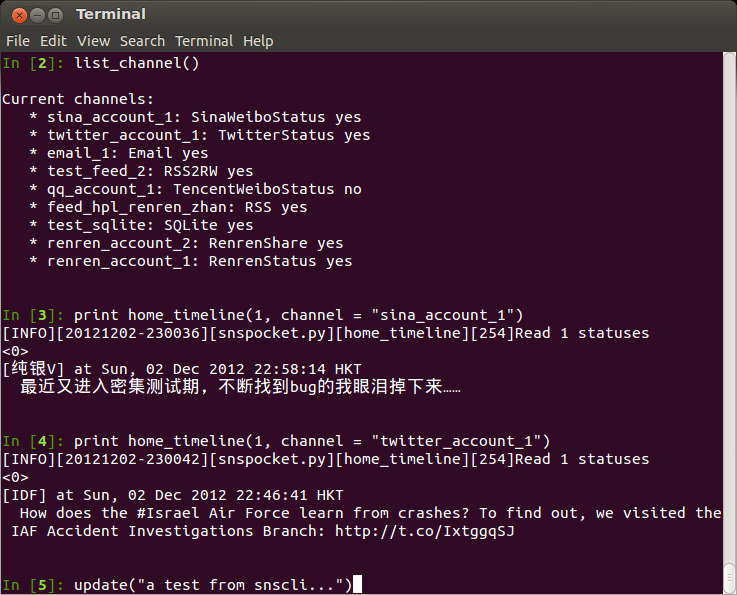
\includegraphics[width=0.7\linewidth]{../pic/snscli.png}
%	\caption{Command Line Interface of SNSAPI}
%\end{figure}
%
%%\begin{figure}[t!]
%%	\centering
%%	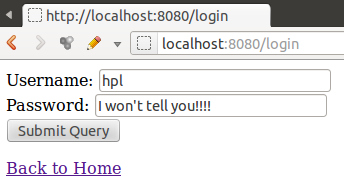
\includegraphics[width=0.7\linewidth]{../pic/srfe_login.png}
%%	\caption{Command Line Interface of SNSAPI}
%%\end{figure}
%
%\begin{figure}[t!]
%	\centering
%	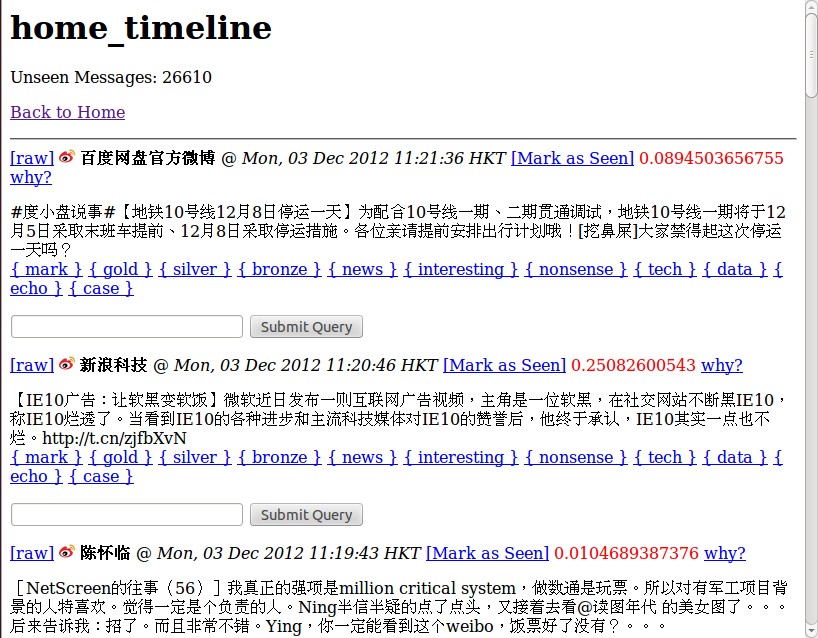
\includegraphics[width=0.7\linewidth]{../pic/srfe_home_timeline.png}
%	\caption{Command Line Interface of SNSAPI}
%\end{figure}
%
%\begin{figure}[t!]
%	\centering
%	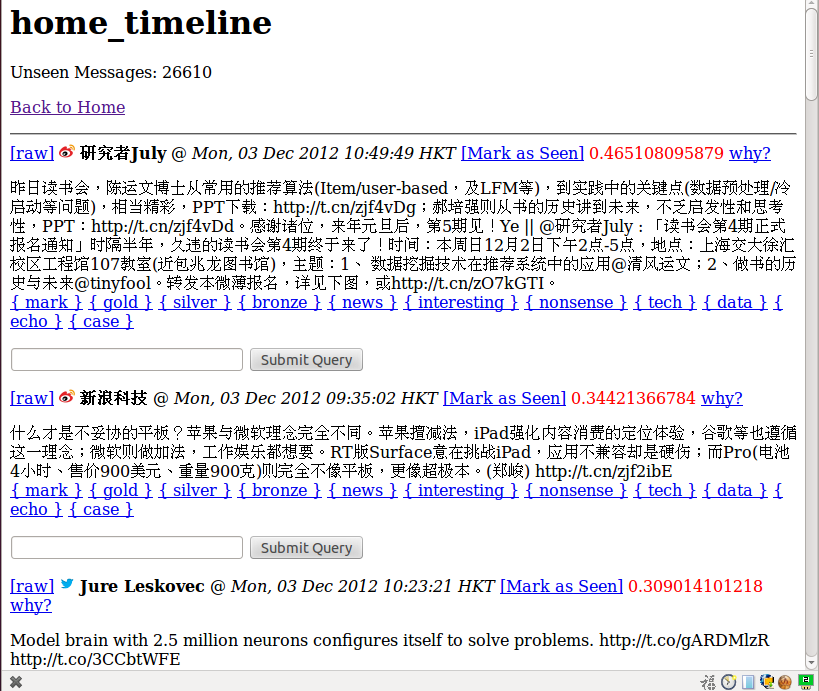
\includegraphics[width=0.7\linewidth]{../pic/srfe_ranked_timeline.png}
%	\caption{Command Line Interface of SNSAPI}
%\end{figure}


\section{Formulation}
\label{sec:Formulation}

In this section, we discuss how we formulate a personalized ranking problem. 
Bear in mind that our ultimate goal is to make 
cross-platform message routing efficient. 
Now the engineering problem has been solved by SNSAPI and \gls{srfe}. 
Next is to design proper machine learning algorithms to make this done automatically. 
In this section, we first discuss the impossibility of 
complete auto forwarding algorithms. 
Then we discuss the problems arise from classification formulation. 
Last, we propose a regression model with user preference constraints. 

\subsection{Impossibility of Auto Forwarding}
\label{sec:Impossibility of Auto Forwarding}

The most aggressive goal of SNSRouter is to make forwarding decisions automatically. 
However, after one month trial, we argue that this is impossible \textbf{in general}. 
By analyzing the real traces (167 forwarded messages out of 7.5K ``seen'' messages), 
we can qualitatively conclude that the forward decision is made by 
considering the following factors:
\begin{itemize}
	\item Quality. 
		This usually applies to knowledge sharing and discussion. 
	\item Novelty (freshness). 
		This usually applies to news. 
	\item Authority. 
		This usually applies to news. 
	\item Degree of wisdom. 
		This usually applies to twisdom 
		(tweet-wisdom: refer to those short but philosophy enlightening pieces)
\end{itemize}

Although people have different tastes, the former three factors
may be captured by the machine. 
However, when one looks into the traces, there are more messages 
of the same (even higher) quality, novelty, and authority. 
Why doesn't the user forward them? 
The user's consideration is beyond those factors, like
``I have already forwarded 5 messages today; 
I don't want to flood my friend;
This message is good but I'm not going to forward it''. 
Other examples are like temporary shift of interest. 
Those factors are hard to capture for machines.

Another issue is that forward operation is sparse among all other operations. 
The author is devoted to this project and mark training data every day, 
so 167 out of 7.5K forwarded messages are collected after one month. 
This rate is much higher than ordinary usage of \gls{sns}'s. 
Towards this end, it is very easy for one algorithm to overfit the training samples. 
For example, one algorithm will find the following piece of knowledge 
statistically significant:
``Only messages originated during daytime is valuable enough for Pili to forward''.
Obviously, this is not the case. 
I will miss many good messages posted on Twitter by someone 
at the other side of the earth!
The reason why this rule is statistically significant is that 
I do not have a ranking engine to bring night messages to the front 
in the initial several weeks. 

We argue that complete automatic forwarding decision is impossible in general. 
Human users must review the messages and decide whether to forward. 
Nevertheless, we can develop some assistant tools to 
help human make decision more efficiently. 


\subsection{The Problem of Classification Formulation}
\label{sec:The Problem of Classification}

Suppose we have $N$ messages $m_1, m_2, \ldots, m_N$. 
We can extract some features of the messages somehow:
(sample features are discussed in evaluation section)
\begin{equation}
	\tran{X} = [x_1, x_2, \ldots, x_N]
\end{equation}
where $x_i \in \mathbb{R}^K$. 
Besides, from the Web UI, users can assign tags to each message. 
The relation between messages and tags is multiple-to-multiple. 
For simplicity of discussion, 
let's assume each message has at most one tag
(technically, we can make this true by creating auxiliary tags no 
matter what is the user's interpretation of the main tags). 
For those messages seen by the user by not tagged, 
we assign a ``null'' tag for it. 
Then every seen message has exactly one tag. 
We denote the tag of message $i$ by $t_i$. 
Our first formulation is a classification problem. 
That is, given $X$, try to predict $t_i$ using certain classifiers. 
If this can be done reasonably, users can make decisions based 
on predicted tags and the efficiency is improved. 

We dumped data into arff format and tried two 
commonly used classifiers using Weka \cite{weka}: 
Logit Classifier and J48 decision tree. 
In the experiments, we use Weka's default parameters and avoid any tuning. 
This is because we don't want our ranking algorithm to be the game of machine learning researchers. 
The user's knowledge in machine learning only affects what features he can extract 
but not the quality a learner is trained. 

The accuracy of Logit classifier is only 78.5526\%, 
which is not competitive.
The overall accuracy of J48 is 87.3684\%
and is comparable to our later proposals. 
Although the accuracy is high, 
the rules generate by J48 is very complex, 
and the user can assert that they are ``incorrect'' by a glance. 
We present more data in \textbf{Appendix \ref{sec:app_Classification}}, 
e.g. the confusion matrix, sample branch of the tree, etc. 

Besides the above algorithmic concerns,
classification formulation has other problems:

\begin{itemize}
	\item Hard cut rule. 
		Classifiers set hard cut rule for each class. 
		They usually do not output a likelihood or any equivalence.
		This cause problem when there is one message lie close to 
		``news'' and ``interesting'' in the feature space, 
		but not close enough to any one of them. 
		This message will be treated as ``null'' by nature. 
		However it could be both new and interesting. 
		Although intermediate stage of those classifiers may calculate 
		such values (e.g. posterior in Naive Bayes, ``likelihood'' in Logit, etc), 
		tapping into the already packaged algorithm is needed. 
	\item Human can only process sequentially. 
		In the last subsection, we argued that human has to be the 
		last judge no matter what algorithm is used. 
		If human can only process sequentially, 
		the combined machine+human decision process is also sequential. 
		There is no need to perform very accurate classification.
		According to our philosophy, 
		we should avoid solving this more than necessary problem. 
		On the contrary, if we can order the messages reasonably, 
		this is already good enough for human decision stage. 
\end{itemize}

Based on these observations, we proceed to propose a regression formulation. 

\subsection{Regression Formulation}
\label{sec:Regression Formulation}

Now we have extracted features for messages, $X$. 
Our goal is to rank them properly. 
Bear in mind that this is not a pure offline research experiment. 
New messages are coming in continuously and 
users can request timeline from Web UI at any time at any frequency
(subject to human's Actions Per Minute). 
We don't want to rerank all the messages 
every time when new ones come in and
return the top messages to the user. 
We want to make the query stage efficient. 
One simple solution is to assign a score to a message when it comes in, 
and store the score as a column in database. 
In the query stage, one only need to add an ``ORDER BY'' clause to enable ranking. 
This is standard in database practice and can be done very efficiently. 

How to map features to a single score? 
Our first thought is of course linear combination, i.e. $Xw$. 
For one thing, non linear combination can be casted 
to linear combination by extending the dimension of features. 
For another thing, output of linear combination is highly interpretable, 
e.g. ``+10 if the message comes from Pili'', 
``+5 if the message is about social computing'', etc. 
When talking about ``enough'' features, 
we do not mean the more the better. 
We indeed mean to incorporate more domain knowledge, 
which is possessed by the user
(not the most clever machine learning researcher). 
Then we get the following regression formulation:
\begin{eqnarray}
	\minimize_{w} && ||y - Xw||_2^2 
\end{eqnarray}
where $y_i$ is the score for message $i$. 
If we can find a set of weights $w$ that combines to $y$
very well on training data, 
it is reasonable to expect they perform similarly well 
on future incoming messages. 
Then our ranking flow is:
1) New message comes in; 
2) Extract features;
3) Use learned $w$ to generate a score, $\hat{y}_i = \tran{x_i} w$;
4) Store $\hat{y}_i$ in DB; 
5) In query stage, sort messages by $\hat{y}_i$.

One direct difficulty is that $y$ is unknown and 
it is very hard for users to generate training $y$'s consistently. 
Another problem is that when user's interest shifts, 
he/she has to regrade the messages and train the weights again. 
This regrading process can be tedious for a user. 
Step back a little, we think it is reasonable to ask users to
tell their preference between two messages. 
This leads to the following formulation:
\begin{eqnarray}
	\minimize_{y,w} && ||y - Xw||_2^2 \\
	\text{s.t.} && y_i > y_j, \; \forall (m_i,m_j) \in E
\end{eqnarray}
where $E$ is a set of tuples $(i,j)$ meaning message $i$ is preferred than $j$. 
Note that $y$ in this formulation is unknown variable. 
This makes it different from ordinary regression. 
Besides, $E$ is only a partial ordering, so this is not ordinal regression problem. 
After some literature survey, we did not find similar standard problems. 
Towards this end, we will temporarily term this formulation as 
{\bf Rank Preserving Regression (RPR)}.  
Details on how to obtain $E$ is described in 
\rsec{\ref{sec:Induce Preference Relations on Graph}}. 

\section{Algorithm Design}
\label{sec:Algorithm Design}

In this section, we design the algorithm to train the RPR model. 
We first discuss how the preference constraints $E$ are obtained. 
Then we discuss how to tackle with the optimization problem. 
Besides algorithmic considerations, 
there are also some practical considerations. 
These observations lead to the final choice -- Stochastic Gradient Descent. 

\subsection{Induce Preference Relations on Graph}
\label{sec:Induce Preference Relations on Graph}

\begin{figure}[t!]
	\centering
	\includegraphics[width=0.7\linewidth]{../pic/graph-induction.pdf}
	\caption{Graph Induction of Preference Constraint}
	\label{fig:graph_induction}
\end{figure}

\rfig{\ref{fig:graph_induction}} illustrates how preference constraints $E$ are derived. 
Ovals stand for user defined tags. 
Solid arrows are user specified preference (through a json configuration file).
Note that no matter what is the meaning of the tags for a user, 
he/she should be able to tell which tag is preferred. 
One can just ask himself/herself some questions. 
If I only have 1 minute today, what type of messages do I want to view?
If I have 1 more minute, what other types do I want to view next? 
In this way, users can specify some partial ordering of the tags.

We denote $T_u \succeq T_v$ if tag $T_u$ is preferred than $T_v$. 
We construct the tag graph $G_T = <T, P>$, 
where $T$ is the set of tags and 
$P = \{(T_u,T_v)| T_u \succeq T_v\}$. 
On this directed graph, we can induce more partial orderings. 
More concretely, if there exists a path from $T_x$ to $T_y$, 
we know $T_x \succeq T_y$. 
Since the tag graph is so small, 
we simply invoke Floyd algorithm \cite{wiki_floyd}
to induce those path preferences without customizing on our own. 

Now we collect all path preferences in one set $P_I$
(meaning Induced Preference). 
Note that edge can be treated as length-1 path, so $P \subset P_I$. 
Then we can define message graph $G_M = <M, E>$, 
where $M = \{m_1, m_2, \ldots, m_N\}$ is the set of all messages
and $E = \{(m_i,m_j)| (t_i, t_j) \in P_I\}$ 
encode a partial ordering of the messages. 

We remark that this tag based preference induction is flexible. 
It provides different level of granularities. 
If one only needs coarse-grained ordering, 
he only needs to add two tags like ``good'' and ``bad''. 
One can also provide a set of fine-grained tags in a nested manner. 
e.g. for those tagged as ``good'', he can further tag 
``machine learning'', ``social computing'', etc. 
At first, when there is only a little training samples, 
he can configure only one user-specified preference, 
i.e. ``good'' $\succeq$ ``bad''.
Later when more training samples are available, 
he can add another line of configuration:
``machine learning'' $\succeq$ ``social computing''. 
If his interest shifts one day, he simply change this line to:
``social computing'' $\succeq$ ``machine learning''. 

\subsection{Straight Optimization Solver}
\label{sec:Straight Optimization Solver}

%Existing solvers?
%Ordinal regression?
%Isotonic regression?

The RPR model is in essence a Quadratic Programming (QP). 
There are many existing solvers and 
we can find some Python implementations 
(e.g. cvxpy which solves a superset of problems). 
However, the QP approach has the following problems:
\begin{itemize}
	\item QP solver introduces more dependencies in our project, 
		making it more difficult to port to other platforms. 
	\item Solving QP is costly, 
		if one want to run the algorithm on mobile devices. 
		This is true for both deploying dependent libraries and executing the algorithm.
	\item Plain QP implementation only supports batch optimization. 
		In our problem, $m_i$ comes continuously and $E$ is also evolving. 
		If we want to capture time variant user interest, we must 
		solve QP in an incremental fashion. 
\end{itemize}

%In order to tackle with this problem efficiently, 
%we have to do some transformation. 

With those practical considerations, we seek for 
better training approaches by proper problem transformation. 

\subsection{Problem Transformation}
\label{sec:Problem Transformation}

We first convert the inequality preference constraints 
into equality constraints using indicator function:
%write down the Lagrangian dual 
\begin{eqnarray}
	\minimize_{y,w} && ||y - Xw||_2^2 \\
		\text{s.t.} && I[y_i > y_j] = 1, \; \forall (m_i,m_j) \in E
\end{eqnarray}
where $I[.]$ is the indicator function:
\begin{equation}
	I[x] = \left\lbrace 
	\begin{matrix}
		1 & \text{x is True} \\
		0 & \text{x is False}
	\end{matrix}
	\right.
\end{equation}
Since $I[.]$ only takes 0 or 1, 
the previous optimization is equivalent to the following form:
\begin{eqnarray}
	\minimize_{y,w} && ||y - Xw||_2^2 \\
	\text{s.t.} && 1 - I[y_i > y_j] \le 0, \; \forall (m_i,m_j) \in E
\end{eqnarray}
The Lagrangian of this problem is:
\begin{equation}
	L(y,w,\mu) = ||y - Xw||_2^2 + \sum_{k=1}^{|E|}\mu_k (1 - I[y_i > y_j])
\end{equation}
We can lowerbound the optimal value of the 
original problem by solving the 
Lagrangian dual problem:
\begin{equation}
	v_d^* = \sup_{\mu \ge 0} \inf_{y,w} L(y,w,\mu)
	\label{eq:lag_supinf}
\end{equation}
The point $(\bar{y}, \bar{w}, \bar{\mu})$ which attains the $v_d^*$ 
MAY be approximately an optimizer for the original problem. 
Note that this point does not necessarily be primal optimizer 
because primal feasibility may be violated 
and Lagrangian duality gap is not zero in general. 

To solve the Lagrangian dual problem is still hard. 
Instead of exploring the whole space of $(y, w, \mu)$, 
we restrict ourselves to a family of $(y, w, \mu)$, which is easier to optimize. 
We impose the following additional constraints:
\begin{eqnarray}
	y &=& Xw \\
\mu_i &=& \lambda, \forall i = 1,2, \ldots, |E| \\
 \lambda &\ge& 0
\end{eqnarray}
Then we have:
\begin{equation}
	\tilde{L}(y,w,\mu) = \lambda \sum_{k=1}^{|E|}(1 - I[y_i > y_j])
\end{equation}
The supinf problem of \req{\ref{eq:lag_supinf}} becomes the following optimization:
\begin{eqnarray}
	\minimize_{y,w} && \sum_{(m_i,m_j) \in E} 1 - I[y_i > y_j] \\
	\text{s.t.} && y = Xw
\end{eqnarray}
Note that the constraint can be plugged back to objective, 
so the objective is essentially a function in $w$ 
and the whole problem is an unconstrained programming. 
To make the notation less cluttered, we keep the current form. 
To this point, we reduce variables from $(N +K)$ to $K$, 
which is significant in practice. 
Then it is possible to leverage first-order optimization methods, 
which are usually easy to implement. 

\subsection{Gradient Descent}
\label{sec:Gradient Descent}

%We denote the objective by $f(w)$, which is defined by:
%\begin{equation}
%	f(w) \equiv \sum_{(i,j) \in E} 1 - I[y_i > y_j] \\
%\end{equation}
The standard practice to deal with indicator function is approximation by Sigmoid function:
\begin{equation}
	S(x) = \frac{1}{1+e^{- \beta x}}
\end{equation}
where we add a scaling factor $\beta$ to control the approximation rate. 
As $\alpha$ goes larger and larger, $S(x)$ approximates $I(x)$ better. 
Now we define
\begin{equation}
	f(w) \equiv \sum_{(i,j) \in E} 1 - S(y_i - y_j) \\
\end{equation}
where $y_i = (Xw)_i$ and $(i,j) \in E$ is a shorthand notation for $(m_i, m_j) \in E$. 

The gradient of $f(w)$ is: 
\begin{equation}
	\nabla f(w) = \sum_{(i,j) \in E} \nabla f_{ij}(w) 
\end{equation}
where
\begin{equation}
	\nabla f_{ij}(w) = \beta (1-S(y_i - y_j))S(y_i-y_j)(x_j-x_i)
\end{equation}
Then we can use standard Gradient Descent (GD) to minimize $f(w)$. 

\subsection{Stochastic Gradient Descent}
\label{sec:Stochastic Gradient Descent}

One key observation is that the full gradient $\nabla f(w)$ 
is the summation of per pair partial gradients $\nabla f_{ij}(w)$. 
To perform one step of GD, one needs to sum over $|E| = O(N^2)$ terms.
This is very costly when $N$ goes large. 
Luckily, this summation structure fits Stochastic Gradient Descent (SGD) \cite{wiki_sgd} very well. 
Then we can sample a set of preference relations $E_s \subset E$ 
with $ |E_s| \ll |E| $
and compute a ``stochastic'' gradient:
\begin{equation}
	\nabla f_{E_s}(w) = \sum_{(i,j) \in E_s} \nabla f_{ij}(w) 
\end{equation}
We walk along $-\nabla f_{E_s}(w)$ for certain step size $\alpha$. 
Probabilistically, SGD has similar effect to GD. 
This method is quite popular in the recent years' development of recommender systems. 
From our experience, it is much easier to set step size in SGD than GD. 

In one extreme, we can implement SGD with $|E_s| = 1$. 
Our implementation of SGD can be summarized in \ralg{\ref{alg:rpr_sgd}}. 

\begin{algorithm}[htb]
	\caption{RPR Training Using SGD}
	\label{alg:rpr_sgd}
	\begin{algorithmic}[1]
		\REQUIRE features $X$, initial weights $w^0$, 
		\\ step size $\alpha$, number of rounds $R$
		\ENSURE final weights: $w^{R}$ 
		\STATE $k=1$
		\WHILE{$k \le R$}
		\STATE Sample a pair of preference relation $(i,j)$ 
		\STATE $g_{ij} \leftarrow \nabla f_{ij}(w^{k-1})$
		\STATE $w^{k} \leftarrow w^{k-1} - \alpha g_{ij}$
		\STATE $k \leftarrow k + 1$
		\ENDWHILE
	\end{algorithmic}
\end{algorithm}

\section{Evaluation}
\label{sec:Evaluation}

In this section, we evaluate our RPR-SGD proposal. 
We first introduce the data set collected in a time span slightly more than one month. 
Then we propose to use Kendall's tau correlation coefficient as a metric. 
Performance v.s. complexity of the algorithm is evaluated
with a set of preliminary features.  
We also use real feedback to show that user efficiency is significantly improved. 
Next, we inject noise feature to show the robustness of RPR-SGD. 
Last, we use a case study to demonstrate how easy it is to 
incorporate a new feature and show the adaptive learning behaviour of RPR-SGD. 

\subsection{Pili's Data Set}
\label{sec:Pili's Data Set}

Pili has been running \gls{srfe} for over one month to collect real traces. 
\rtbl{\ref{tbl:dataset}} summarizes some basic statistics. 
We derive training and testing preference relations in the following way:
1) Select out all tagged messages (about 900); 
2) Sample same number of untagged messages (about 900) and assign them ``null'' tag;
3) Divide the candidate messages (about 1.8K) into training and testing sets randomly;
4) Use graph induction to form $G_{M_{\text{train}}}$ and $G_{M_{\text{test}}}$, 
where ${M_{\text{train}}}$ is training set and ${M_{\text{test}}}$ is testing set. 
Altogether, there are more than 200K relations in both training and testing sets. 

\begin{table}[htb]
	\centering
	\caption{Basic Statistics of Pili's Data Set}
	\label{tbl:dataset}
	\begin{tabular}{l|c}
		\hline
		Item & Value \\
		\hline
		\# of total messages & 32533\\
		\# of seen messages & 7553\\
		\# of tagged messages & 924\\
		\# of forwarded messages & 167\\
		\# of derived pairs (training) & 231540\\
		\# of derived pairs (testing) & 229009\\
		\# of features (+1 noise) & 15\\
		\hline
	\end{tabular}
\end{table}

\subsection{Criterion}
\label{sec:Criterion}

Kendall's tau correlation coefficient \cite{wiki_kendall} is a good measure of rank. 
The modified version for our problem is defined as:
\begin{equation}
	K = \frac{
	\sum_{(i,j) \in {E_{\text{test}}} }{I[\hat{y}_i>\hat{y}_j]} 
	- \sum_{(i,j)\in {E_{\text{test}}} }{I[\hat{y}_j>\hat{y}_i]}  }
	{|E_{\text{test}}|}
\end{equation}
where $\hat{y}_i$ is the predicted score of message $i$ using the learned weights $w$
and $E_{\text{test}}$ is the set of edges in $G_{M_{\text{test}}}$. 
The first summation in numerator counts the number pairs whose relation is preserved. 
The second summation in numerator counts the number pairs whose relation is violated. 
The denominator is the total number of relations in our concern. 
Given this definition, we know that $K \in [-1, 1]$ and the larger the better. 
This is in accordance with the notion of correlation. 
When $\hat{y}_i$'s are assigned randomly, we can expect $K = 0$. 
In the following discussions, we also call this measure Kendall's score for short. 

\subsection{Sample Features}
\label{sec:Sample Features}

We argue that our RPR-SGD framework is easy to use, 
so we do not try very hard to extract advanced features
(although they are apparently future work). 
\rtbl{\ref{tbl:feature}} summarizes our sample features extracted by our first user (Pili). 
He is not an expert in text analysis like topic mining, sentiment analysis, etc. 
Writing the logic to extract those features adds up to 
approximately (maybe slightly more than) one day's work. 

\begin{table}[htb]
	\caption{Features}
	\label{tbl:feature}
	\centering
	\begin{tabular}{l|p{0.5\linewidth}}
		\hline
		Name & Description \\
		\hline
		noise & Random variable in [0,1]\\
		 echo & \{0, 1\}: Whether the message is from myself\\
		contain\_link & Whether the message contains text link\\
		topic\_interesting & TF*IDF for ``interesting'' \\
		topic\_tech & TF*IDF for ``mark'' ``gold'' ``silver'' ``bronze''\\
		topic\_news & TF*IDF for ``news''\\
		topic\_nonsense & TF*IDF for ``nonsense'' ``shit''\\
		user\_interesting & As above; Treat ``user'' as ``term''\\
		user\_tech & As above\\
		user\_news & As above\\
		user\_nonsense & As above\\
		text\_len & Length of all message (original + retweet)\\
		text\_len\_clean & Length without emoji, ``@xxx'' and puctuation\\
		text\_orig\_len & Length of original message\\
		\hline
	\end{tabular}
\end{table}

Most of the features should be self-explanatory. 
We only elaborate the ``topic\_X'' and ``user\_X'' features a bit. 
We first discuss how we extract ``topic\_news'' from messages. 
TF stands for Term Frequency and IDF stands for Inverse Document Frequency. 
Those two terms are borrowed from Information Retrieval field. 
We perform word segmentation (a vital step for Chinese messages) 
on all incoming messages and get the 
frequency that each term appears in those messages (DF).
Similarly, we can first select all messages tagged as ``news'' by the Pili
and count the term frequency (TF). 
The intuition is that the more frequent a term appears in ``news'' category, 
the more representative it is for this category; 
Also, the more frequent a term appears in all messages, 
the less representative it is for this category. 
The simplest way to implement this notion is TF times IDF. 
We can extract other topics in the same way. 
With a strong domain knowledge, the users can group several tags and extract topic together. 
When one new message comes in, we sum up all the TF*IDF values of its terms. 
Likewise, if we treat the sender of each message as a ``term'',
we can compute a TF*IDF value for users,
namely how likely a user will post certain topic. 

We remark that the topic mining part is very elementary. 
One can use more advanced tools like WordNet, Ontology, etc. 
As an additional note, the word segmentation we used is 
Maximum Matching Segmentation (MMSeg), and our dictionary is 
simply a merge of pymmseg-cpp and SogoW (Sogo dict dating back to 2006). 
Many new terms, especially cyber phrases, can not be correctly segmented. 

\subsection{Performance and Complexity}
\label{sec:Performance and Complexity}

We implemented SGD in SNSRouter project using Python straightforwardly. 
The code has not been optimized.
\rtbl{\ref{tbl:sgd_train}} shows the performance v.s. complexity. 
Step size is chosen as $\alpha = 10^{-2}$. 
When more rounds of SGD is performed, the Kendall's score becomes higher. 
In this setting, testing K becomes larger than $0.7$ after 
several dozens of thousand iterations. 
This is substantial improvement compared to unranked version, 
meaning $85\%$ pairs are in correct order 
(i.e. $K = (0.85 |E| - 0.15 |E|) / |E|$). 
From the data, we can see that SGD scales well. 
We also implemented GD.
Under the same settings, 
GD costs about 30s in one step and 
needs about 15 steps to walk a point with $K \approx 0.75$. 
The author is confident that the SGD algorithm can be 
an order of magnitude faster by only code level optimization. 
For the time being, we leave it to the future work. 

\begin{table}[htb]
	\centering
	\caption{Training with SGD}
	\label{tbl:sgd_train}
	\begin{tabular}{c|c|c|c}
	\hline
	Item & 1. & 2. & 3. \\
	\hline
	\# of rounds of SGD & 200,000 & 400,000 & 1,000,000\\
	Wall clock time & 32.63s & 60.81s & 159.57s\\
	Kendall's score (training) & 0.8178 & 0.8349 & 0.8414\\
	Kendall's score (testing) & 0.7598 & 0.7758 & 0.7865\\
	\hline
	\end{tabular}
\end{table}

We also remark that:
\begin{itemize}
	\item Larger $\alpha$ make SGD go faster but the oscillation around 
		optimal point is larger. 
		Small $\alpha$ is conservative so that it goes slower but is more stable. 
		Users can configure different step size 
		according to his/her demand and ability of device. 
	\item Exactly optimizing the weights is not needed, 
		as we argued in the formulation section. 
		A set of coarsely tuned weights is already good enough
		to boost the user's efficiency. 
		Users who are conscious of their domain knowledge 
		can set the weights manually (or use it as initial point $w^0$). 
		The first user (Pili) tried to manually craft a set of weights
		before any learner algorithm (e.g. SGD) is available. 
		He spent 1 minute and came up with a weighting scheme 
		which reaches a Kendall's score of $0.68$. 
		As the data set varies, this score may not be comparative to the above scores. 
		Nevertheless, he can tell that the ranked timeline is 
		already significantly better than raw timeline. 
\end{itemize}


%\begin{itemize}
%	\item Scale linearly
%	\item Online learning is possible
%	\item Easy configuration
%	\item Easy to add new features
%\end{itemize}

\subsection{Improved User Efficiency}
\label{sec:Improved User Efficiency}

We present the user feedback in \rtbl{\ref{tbl:user_eff}} to show RPR-SGD 
improves user efficiency significantly. 
We divide time period by weeks to absorb natural variance
such as workday v.s. weekend, day v.s. night, etc. 
This deployment connects to Renren, SinaWeibo, TencentWeibo, SQLite, Gmail, and several other RSS feeds. 
``All'' is the total number of messages fetched during the experiment time. 
``Seen'' is the total number of messages seen by the user
(flagged as ``seen'' from \gls{srfe}). 
``Value'' means useful information to the user. 
As a rough estimation, we regard the following tags as ``Value'':
``gold'', ``silver'', ``bronze'', ``mark'', ``news'', ``interesting''
(As is shown in \rfig{\ref{fig:graph_induction}}, they have ``$\succeq$'' relation to ``null''). 
The last column ``V/S'' counts the ratio between ``Value'' and ``Seen''. 

\begin{table}[htb]
	\centering
	\caption{User Efficiency Evaluation}
	\label{tbl:user_eff}
	\begin{tabular}{c|c|c|c|c|c}
		\hline
		No. & Period & All & Seen & Value & V/S \\
		\hline
		1 & Nov 13 - Nov 20 & 6578 & 1489 & 114 & 7.6561\% \\
		2 & Nov 20 - Nov 27 & 9040 & 1544 & 138 & 8.9378\% \\
		3 & Nov 27 - Dec 04 & 8472 & 846 & 184 & 21.749\% \\
		4 & Dec 04 - Dec 11 & 8243 & 225 & 56 & 24.889\% \\
		\hline
	\end{tabular}
\end{table}

It is obvious that RPR-SGD improves user efficiency. 
To help the readers truthfully interpret the presented result, 
we should note the following facts:
\begin{itemize}
	\item Preliminary reranking test was brought online at Nov 26. 
		One can see the V/S ratio is already slightly higher in week2. 
	\item In week1, the \gls{srfe} is not running continuously day and night, 
		because it is in the intensive debug period. 
		Number of total messages is significantly smaller. 
		This is only the number of messages collected during Pili's working time. 
	\item Compared to week2, week3 and week4 have fewer number of total messages. 
		This is because connection from CUHK campus to TencentWeibo API server failed since about Dec 1. 
		We observed the unstability issue of TecentWeibo API server several times 
		prior to SNS-Router project. 
		This is out of our debugging ability. 
	\item In week3 and week4, the user was not fully exposed to ranked timeline. 
		He went back to ordinary timeline from time to time. 
		This is to serve more unbiased samples for the algorithm. 
		It will lower ``V/S'' somehow, but bring positive effect in the long run. 
	\item When viewing the ranked timeline, user's criterion will be subconsciously higher. 
		This is natural psychological effect. 
		If the baseline is better, people tend to be more strict. 
		Even with perfect ranking, people are unlikely to tag
		most of the top entries as valuable. 
	\item We observe that duplication is a major cause to make ``V/S'' 
		value look poorer than Kendall's score. 
		Many times, the same information was tweeted by different sources using different wording. 
		If it is valuable (according to our trained weighting scheme), 
		all those messages are ranked high. 
		However, the user may only ``mark'' one of them for future retrieval. 
		We will discuss more on this aspect in the future work section. 
\end{itemize}

In total, we find RPR-SGD can improve user efficiency substantially. 
It performs good in screening off noisy messages. 
As to duplicated high quality messages, more work has to be done 
to improve user efficiency to a higher level. 

\subsection{Robustness}
\label{sec:Robustness}

In this experiment, we test how robust our algorithm is to noise. 
This is important measurement because we expect user to extract features for themselves. 
If their feature is not informative under RPR model or is nearly to noise, 
our weighting should not deviate too much. 
Being robust is the first step.
In the future work, we can add automatic feature selection techniques.

We start with features listed in \rtbl{\ref{tbl:feature}} without ``noise'', 
and run enough steps of SGD to get a point with $K>0.8$. 
The absolute values of trained weights for the rest features are all less than 10. 
Then we inject 1 noise feature, which is a random variable $\sim U[0,1]$. 
We initialize the weight of ``noise'' by 10.
\rtbl{\ref{tbl:noise}} shows the training result. 

\begin{table}[htb]
	\centering
	\caption{Robustness Test}
	\label{tbl:noise}
	\begin{tabular}{c|c|c|c}
		\hline 
		& Init & Round=200K & Round=400K \\
		\hline 
		Kendall & 0.0772 & 0.5435 & 0.8060 \\
		 w(noise) & 10.0 & 1.3407 & -0.0132 \\
		\hline
	\end{tabular}
\end{table}

One can see that the Kendall's score is close to 0 initially. 
This is because we initialized ``noise'' with very large weight
and it becomes the dominating factor. 
Random ordering of the messages should result in $K \approx 0$. 
With more steps of SGD, the absolute value of the weight of ``noise'' becomes smaller
and corresponding Kendall's score also improves. 

We have the following remarks:
\begin{itemize}
	\item We can add regularization terms to force non-informative features' 
		weights approach zero. 
		This is left to future work. 
	\item Although the original purpose of ``noise'' feature is just for experimenting, 
		we later find that ``noise'' is a very good feature. 
		With small but not fully negligible weight, 
		it introduces reasonable disturbance into the system, 
		thus providing less biased samples. 
		For example, if the user make posting time a feature, 
		the algorithm may conclude that ``larger timestamp is preferred''.
		This is purely because messages are presented in reverse chronological order on the original timeline
		(where the users mark for training samples). 
		When two messages are similar, only the first one ``seen'' by the user are marked. 
		Such self-validation effect can be alleviated by a noise feature. 
\end{itemize}

\subsection{Case Study -- Echo Cancellation}
\label{sec:Case Study -- Echo Cancellation}

In this section, we provide abundant screenshots with detailed steps 
to show how to add a new feature. 
We also present animation of training process to 
give the reader an impression of how RPR-SGD is adapting to new changes.  

We choose Echo Cancellation as an example. 
\gls{sns} users should have noticed that they see their own 
messages on the timeline among others' posts. 
This is true for most platforms. 
We call those messages ``echo''. 
\rfig{\ref{fig:echo_ranked_timeline_before}} shows the ranked timeline before echo cancellation. 
Echo will be more significant when the timeline is ranked: 
1) A rational user is most likely to forward valuable (at least to him/her) messages;
2) The ranking algorithm learns the user's preference and rank those messages higher;
3) When forwarding the message, the user adds some comments, making it 
more valuable (from the algorithms point of view);
4) After fetching new messages, echos are more likely to rank higher. 

\begin{figure}
	\centering
	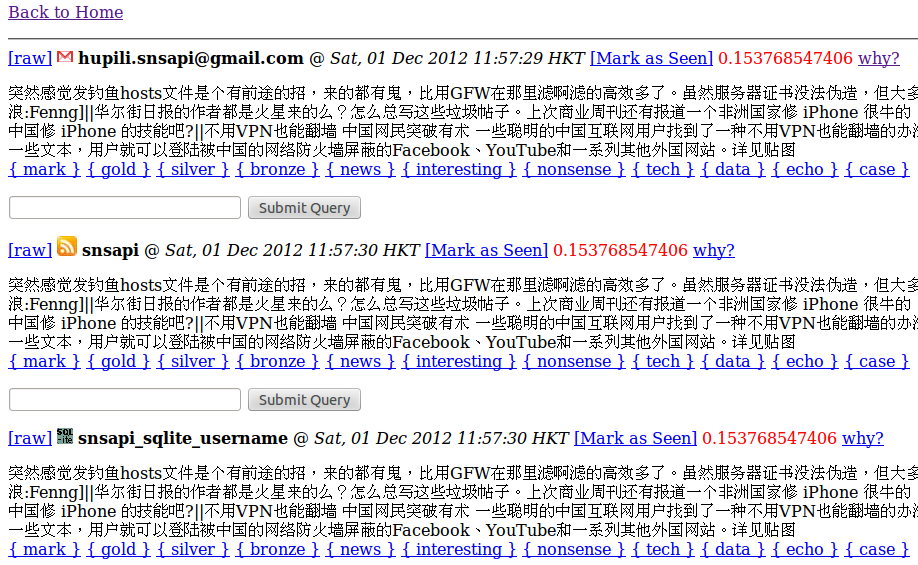
\includegraphics[width=0.9\linewidth]{../pic/echo_ranked_timeline_before.png}
	\caption{Ranked Timeline with Echo}
	\label{fig:echo_ranked_timeline_before}
\end{figure}

We have many ways to cancel echos. 
For example, a programmer will find it very easy 
to use several lines of ``IF'' to achieve this goal. 
This way fits original notion of SNSAPI. 
We just enable the flexibility and let App developer to craft their own logic. 
In SNSRouter project, we are more serious about ranking. 
If one only needs to cancel echos, the straight coding is a good solution. 
However, we can imagine that users have many similar demand, 
e.g. ``rank messages from some people higher'', 
``rank messages containing music links higher'', etc. 
When the ``IF'' tree grows large, it will be hard to manage it efficiently. 
RPR provides the framework so that users only need to tell 
the machine what factor may be important. 
The machine will automatically adjust between different factors. 

%Most platforms will echo the
%message you post there, but they
%do not give you more information.
%We want to SOFTLY cancel them.

Here is the way to to {\bf softly} cancel echos:
\begin{enumerate}
	\item Add tag ``echo'' on the config panel of \gls{srfe}, 
		as is shown in \rfig{\ref{fig:echo_add_tag}}. 
	\item Users go to \gls{srfe} and tag some messages as ``echo''. 
		The user can do this gradually for some time. 
		Or, the user can go to our SQL frontend on \gls{srfe}
		to intentionally select out some messages. 
		In the latter way, users are leveraging their own domain knowledge. 
	\item Specify preference through json config file, 
		as is shown in \rfig{\ref{fig:echo_preference}}. 
		Here we only add one preference relation: ``null'' $\succeq$ ``echo''. 
	\item Add the feature extraction logic as is shown in \rfig{\ref{fig:echo_feature}}. 
		The user simply derives a feature extractor from base class ``FeatureBase''.
		Except for structural codes, this example feature extractor 
		only costs about 10 lines of codes.
		Many of the 15 feature extractors used in previous evaluation are also only several dozens of lines. 
	\item After the above preparation, 
		the weights can be trained automatically. 
		\rfig{\ref{fig:echo_train}} gives an animation of how 
		weights are adapted to the new scenario. 
		To make it less cluttered, we selectively depicted some features for comparison. 
		One can consult the notes in SNSRouter repository for detailed data. 
		The figures show weight of ``echo'' (2nd column) goes negatively
		with more iterations and the other features remain roughly the same. 
\end{enumerate}

%\begin{figure}[htb]
%	\centering
%	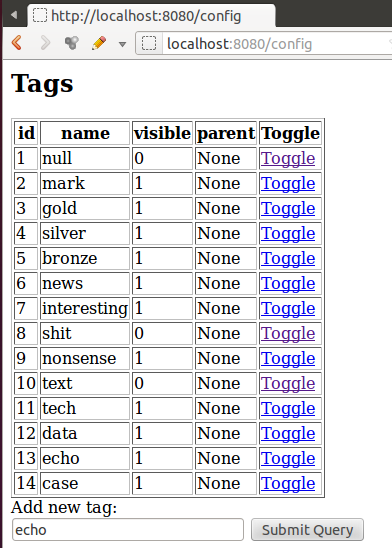
\includegraphics[width=0.5\linewidth]{../pic/echo_add_tag.png}
%	\caption{Add New Tag on Config Panel}
%\end{figure}
%
%\begin{figure}[htb]
%	\centering
%	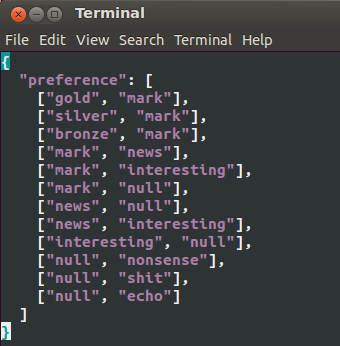
\includegraphics[width=0.6\linewidth]{../pic/echo_preference.png}
%	\caption{Specify Preference for Echo}
%\end{figure}
%
%\begin{figure}[htb]
%	\centering
%	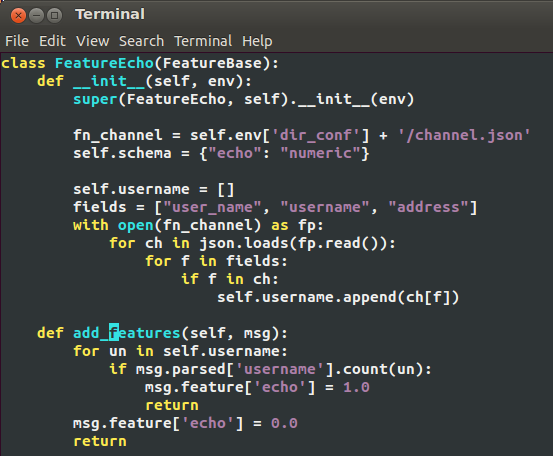
\includegraphics[width=0.7\linewidth]{../pic/echo_feature.png}
%	\caption{Add Feature Extraction Module}
%\end{figure}

\begin{figure*}
	\centering
	%\subfigure[Add New Tag on Config Panel]{%
	\subfigure[Add New Tag]{%
	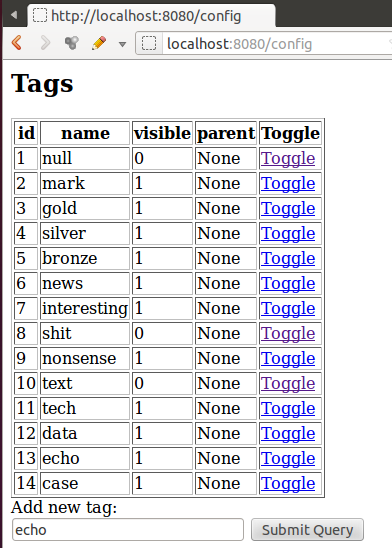
\includegraphics[width=0.21\linewidth]{../pic/echo_add_tag.png}
	\label{fig:echo_add_tag}
	}
	\centering
	\subfigure[Specify Preference for Echo]{%
	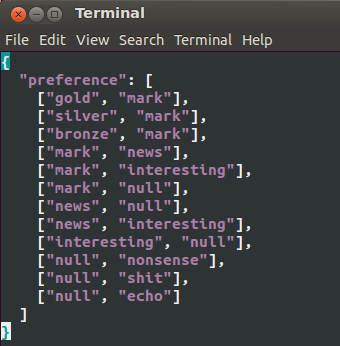
\includegraphics[width=0.29\linewidth]{../pic/echo_preference.png}
	\label{fig:echo_preference}
	}
	\centering
	\subfigure[Add Feature Extraction Module]{%
	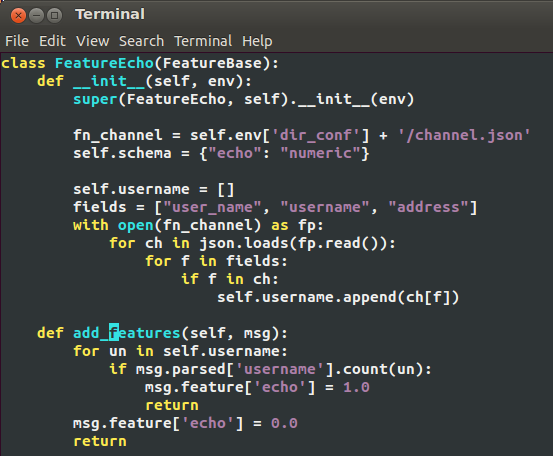
\includegraphics[width=0.36\linewidth]{../pic/echo_feature.png}
	\label{fig:echo_feature}
	}
	\caption{Three Steps to Add New Features}
\end{figure*}

\begin{figure}
	\centering
	\subfigure[Iteration i]{%
	\label{fig:srfe_rankedtimeline}
	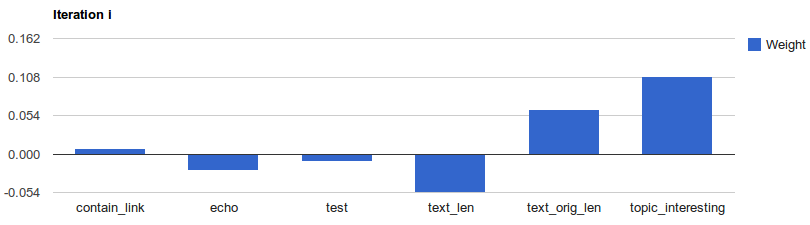
\includegraphics[width=0.7\linewidth]{../pic/echo_gd_i.png}
	}\\%    
	\subfigure[Iteration i+1]{%
	\label{fig:srfe_rankedtimeline}
	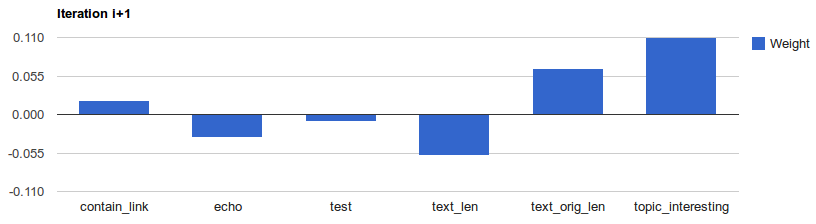
\includegraphics[width=0.7\linewidth]{../pic/echo_gd_i1.png}
	}\\%   
	\subfigure[Iteration i+2]{%
	\label{fig:srfe_rankedtimeline}
	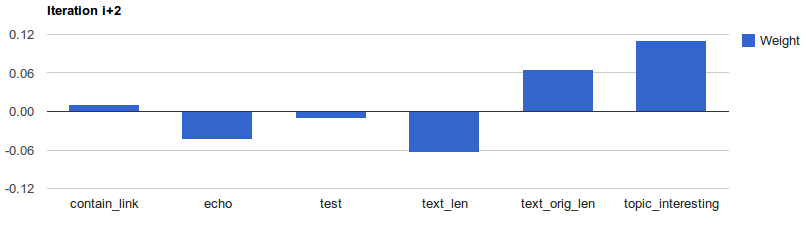
\includegraphics[width=0.7\linewidth]{../pic/echo_gd_i2.png}
	}\\%   
	\caption{Training Echo Feature}
	\label{fig:echo_train}
\end{figure}

%\begin{figure}[h!]
%	\centering
%	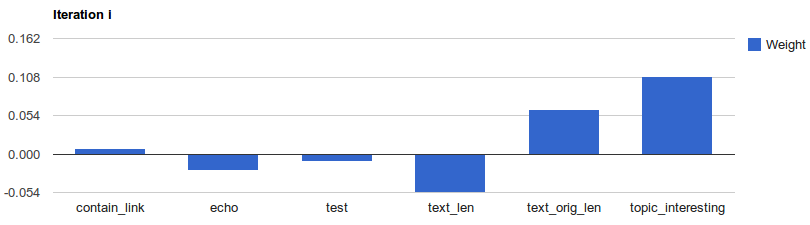
\includegraphics[width=0.7\linewidth]{../pic/echo_gd_i.png}
%	\caption{Add New Tag on Config Panel}
%\end{figure}
%
%\begin{figure}[h!]
%	\centering
%	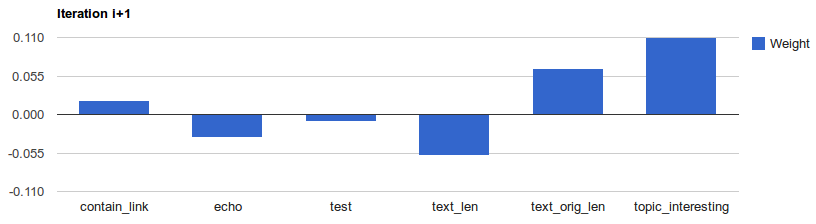
\includegraphics[width=0.7\linewidth]{../pic/echo_gd_i1.png}
%	\caption{Add New Tag on Config Panel}
%\end{figure}
%
%\begin{figure}[h!]
%	\centering
%	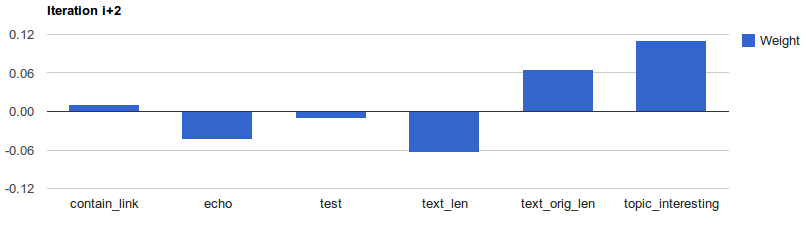
\includegraphics[width=0.7\linewidth]{../pic/echo_gd_i2.png}
%	\caption{Add New Tag on Config Panel}
%\end{figure}


%The weight of ``echo'' feature goes down iteration by iteration. Messages with ``echo=1''
%will be ranked lower. This is auto learned by our RPR-SGD framework.

We remark that the weights adaption shown in \rfig{\ref{fig:echo_train}}
is highly interpretable for the user. 
The ``echo'' feature is either 1 or 0 
and it recognizes echos by comparing sender name with channel configurations. 
Since its weight is negative, 
messages with ``echo=1'' will be ranked lower. 
This agrees with the ``IF'' logic in our first thought. 
The nice property for RPR-SGD is that this weight is trained automatically.  

\section{Conclusion}
\label{sec:Conclusion}

We observe that message forwarding is a major operation on \gls{sns}. 
Cross-platform forwarding behaviour is seldom discussed 
in both industry and academia. 
One main reason is that there is no full solution stack to 
make it automatic or semi-automatic, 
in order for researcher to collect enough data. 
There are also some business considerations discussed in Appendix \ref{sec:Business}.
In this paper, we take an initial step to tackle with the problem 
by leveraging system, algorithm and human in the following steps:

\begin{itemize}
	\item Develop a middleware for heterogeneous SNS's. 
	\item Develop a portable web frontend which supports 
		easy cross-platform message forwarding and personal tagging. 
	\item Collect real data in more than one month time span. 
	\item Propose a flexible algorithm framework (RPR-SGD)
		to personalize incoming message ordering, 
		which boosts the user efficiency. 
	\item Develop some sample feature extraction modules. 
\end{itemize}

Note that the usage of SNSRouter is not restricted to forwarding assistant. 
It can be used as a personal information center 
(with more forthcoming SNSAPI plugins). 
For example, monitor your course webpage and send emails 
to your friends when new slides are posted. 
For another example, follow celebrities on SinaWeibo
so that their messages (including later deleted ones) are all automatically archived. 
This provides a distributed witness force, which help to improve 
their awareness of social responsibility!
\footnote{
	Many celebrities on SinaWeibo act like media. 
	They pursue the speed of dissemination information and the exposure rate. 
	Many of them do not spend a minute to validate the messages they forward. 
	After people find out it is rumor, 
	they just delete the original message quietly 
	without one word of apology. 
	Late comers will only see a sentence in original position:
	``This message is deleted, please consult the customer service for more information''
	(in Chinese). 
	However, the influence is already far spread on the network. 
	I believe, the \gls{osn}'s will be more reliable if many people are running SNSRouter. 
	Under this scenario, those celebrities will think twice before they act. 
	When mistakes are made, they will prefer to fix them rather than hide them. 
}

In total, SNSAPI and SNSRouter are open by design. 
Your imagination combined with our system infrastructure can result in many novel applications. 

\section{Future Work}
\label{sec:Future Work}

In this section, we discuss promising future works. 
Some are directly followed from the discussions in previous sections. 
Some are our visions. 
We discuss from three aspects: system, algorithm and evaluation. 

\subsection{System}
\label{sec:fu_System}

\begin{itemize}
	\item Develop RESTful interface for all components of SNS-Router.
		Then one can outsource computationally intensive training to other servers. 
	\item Add a new platform -- SNSRouter to SNSAPI.
		One can then fetch SNSRouter timeline in the same way as others. 
		In this way, users can use SNSRouter to aggregate multiple channels,
		which is useful to deal with large amount of RSS feeds. 
	\item Build user community.
		We can provide online ``FeatureStore'' and ``LearnerStore''. 
		In this way, users do not have to be constrained to our sample features
		or try to extract anything themselves. 
		They can upload their extractors and download others' extractors. 
		Those components are pluggable by configuration 
		so that better personalization level is reached. 
\end{itemize}

\subsection{Algorithm}
\label{sec:fu_Algorithm}

\begin{itemize}
	\item Add regularization terms. 
		First is to alleviate overfitting and standard L2 norm regularization suffices. 
		Second, we can perform feature selection using L1 regularization first 
		and only train selected features. 
	\item Build advanced feature extractors. 
		In the topic mining part, we used TF*IDF. 
		There is large room to improve. 
		For example, at the startup time,
		the system do not collect enough terms to do TF*IDF.
		If we plug a WordNet into SNSRouter, 
		we can enlarge the term set by diffusion techniques. 
		This also provides a way to smooth term importance and 
		mine hidden (semantical not literal) topic. 
	\item Code level optimization of SGD. 
		As is mentioned in evaluation section, 
		code level optimization for SGD can be done. 
		We can change to ``numpy'' objects to avoid 
		time consuming operations like list traversal. 
		We can also implement a dedicated SGD library in C with Python module encapsulation. 
		To make the code easy to migrate, 
		the current stupid implementation will be kept as default portability consideration. 
		After the users verify everything is going well, 
		they can configure to optimized modules. 
	\item SGD can do online training.
		e.g. one sample in, derive some pairs, do SGD on those pairs.
		In this way, it provides natural time sliding.
		Current SGD implementation in SNSRouter is batch training, 
		which can be triggered by the user. 
		One recent target is to make it online. 
		The difficulty is not at algorithm side. 
		Instead, sliding memory caching is needed to make it possible. 
		Original plain SQLite interface will cause very large overhead. 
	\item Deduplication. 
		As we discussed in evaluation section, 
		deduplication is a major cause to make overall efficiency gain 
		for the users less significant than we expect from Kendall's score. 
		Algorithmic wise, this is a traditional problem in IR. 
		As to our application scenario, 
		we also want to improve the frontend at the same time, 
		so that users can process duplicated messages quickly. 
		For example, we can present similar messages in tree structure
		so that users can``mark as seen'' in a batch. 
\end{itemize}

\subsection{Evaluation}
\label{sec:fu_Evaluation}

More subjective tests are to be done:

\begin{itemize}
	\item We argue the algorithm framework is easy to personalize. 
		In the future work, we will invite more developers 
		who are not machine learning experts to test our system. 
		In this way, we can see how efficient people are 
		after they use our system. 
		More sample extractors can be output in this process. 
\end{itemize}

\section*{Acknowledgements}
\label{sec:Acknowledgements}

SNSAPI is the base of SNSRouter project. 
We would like to thank Junbo Li from BUPT, who is the co-founder of SNSAPI.  
We thank other contributors from Github: Chunliang Lu. 
We also highly appreciate people who answered our technical questions on StackOverflow. 
We thank Xiaoying Tang for her review of this report. 

\bibliographystyle{abbrv}
\input{../reference/gen_bib.bbl}

\appendix 

%\section{Data}
%\label{sec:Data}

\section{Business}
\label{sec:Business}

We tried to upgrade one sample app key on SinaWeibo but failed.
\footnote{See the issue tracker for more details, \url{https://github.com/hupili/snsapi/issues/11}}
The reason is that they forbid cross-platform forwarding applications. 
From a few survey, we summarize some of their business considerations:
\begin{itemize}
	\item Competition. 
		They don't want users just to go to other \gls{osn} but possess 
		the ability to synchronize content back to SinaWeibo.
		They want to lock users in because advertisements are presented on user timeline
		if they access it from web. 
		This is very similar to the old days when you can not 
		transfer cellphone number from one service provider to another. 
		Considering the links established within one platform, 
		users find it difficult to migrate to another platform. 
	\item Censorship. 
		SinaWeibo monitors user content and delete / block / hide messages 
		if they are not appropriate. 
		If multi-platform synchronization is allowed, those messages 
		forwarded to another platform are out of control. 
		In this case, they forbid any form of synchronization
		(even with application and audition). 
\end{itemize}

The first one is out of our consideration. 
The second one is just placing a thin film to slow down the information dissemination process. 
You can not stop users' copy and paste anyway. 

The way they stop such applications is by killing their app keys. 
This is effective if the App developer resort to a closed system 
and hide all details from the user. 
On another hand, we agree that this lowers the barrier for 
ordinary users to use the App. 

Given those observations, we position SNSAPI and 
SNS-Router as developer applications. 
If a user want to use SNSRouter,
he/she may have to spend several minutes 
to apply his/her own app key. 
Then the use of SNSRouter from service provider's point of view is just 
someone testing a new App.
This is the freedom of developers and is in general hard to block. 

\section{Classification}
\label{sec:app_Classification}

As we mentioned in the formulation section, 
classification is one candidate formulation initially. 
We dumped data to arff format and ran some preliminary experiments. 

\subsection{Logit Classifier}
\label{sec:Logit Classifier}

The accuracy that Logit Classifier can reach is 78.5526\%. 
Comparing with the data we presented in evaluation section, 
this performance is not competitive. 
A 0.8 Kendall's score maps back to 90\% correctly ranked pairs. 
Incorrectly classified instances will amplify to larger number of incorrect pairs. 
The confusion matrix is presented in \rfig{\ref{fig:confmat_logit}}. 
We can see that the most confused part is ``news''. 
From the user's point, this is natural. 
When I tagged messages as news, I already realized that 
there were not enough features for ``news''. 
First, they come from a wide spectrum of topics:
politics, military, science, etc. 
It is hard to use topic to judge the ``news''-ness, 
letting alone judge it with our elementary topic miner.

\begin{figure*}[t!]
	\centering
\begin{Verbatim}
   a   b   c   d   e   f   g   h   i   j   k   l   m   n   o   <-- classified as
   5   0   0   0   0   0   0   0   0   0   0   2   0   0   0 |   a = echo
   0   2   0   0   0   0   0   0   0   0   0   0   0   0   0 |   b = case
   0   0   0   0   0   0   0   0   0   0   0   0   0   0   0 |   c = gold
   0   2   0  16   0   0   0   0   0   0   0   2   0   0   0 |   d = interesting
   0   0   0   2  71   0   0   0   7   0   0  15   0   0   0 |   e = nonsense
   0   0   0   0   0   0   0   0   0   0   0   0   0   0   0 |   f = __fake__
   0   0   0   0   0   0  90   0   0   0   1  22   0   0   0 |   g = mark
   0   0   0   0   0   0   0   0   0   0   0   0   0   0   0 |   h = tech
   0   0   0   3   1   0   0   0  10   0   0   0   0   0   0 |   i = shit
   0   0   0   0   0   0   0   0   0   0   0   0   0   0   0 |   j = text
   0   0   0   0   0   0   1   0   0   0  40  76   0   0   0 |   k = news
   2   1   0   4   4   0   4   0   0   0  14 363   0   0   0 |   l = null
   0   0   0   0   0   0   0   0   0   0   0   0   0   0   0 |   m = data
   0   0   0   0   0   0   0   0   0   0   0   0   0   0   0 |   n = silver
   0   0   0   0   0   0   0   0   0   0   0   0   0   0   0 |   o = bronze
\end{Verbatim}
	\caption{Confusion Matrix, Logit Classifier}
	\label{fig:confmat_logit}
\end{figure*}

\subsection{J48 Decision Tree}
\label{sec:J48 Decision Tree}

J48 decision tree can reach an overall accuracy of 87.3684\% (testing). 
This value is very good. 
The confusion matrix is presented in \rfig{\ref{fig:confmat_j48}}. 
One can see that it performs equally well for all classes. 
This is because decision tree can generate arbitrary 
(axis perpendicular) decision boundary. 
We also remark that the training and testing speed for J48 very high. 
All the process is completed in less than 5 seconds. 

\begin{figure*}[t!]
	\centering
\begin{Verbatim}
   a   b   c   d   e   f   g   h   i   j   k   l   m   n   o   <-- classified as
   6   0   0   0   0   0   1   0   0   0   0   0   0   0   0 |   a = echo
   0   2   0   0   0   0   0   0   0   0   0   0   0   0   0 |   b = case
   0   0   0   0   0   0   0   0   0   0   0   0   0   0   0 |   c = gold
   0   0   0  15   0   0   0   0   0   0   0   5   0   0   0 |   d = interesting
   0   0   0   0  70   0   2   0   6   0   1  16   0   0   0 |   e = nonsense
   0   0   0   0   0   0   0   0   0   0   0   0   0   0   0 |   f = __fake__
   0   0   0   0   0   0  94   0   0   0   3  16   0   0   0 |   g = mark
   0   0   0   0   0   0   0   0   0   0   0   0   0   0   0 |   h = tech
   0   0   0   0   1   0   0   0  13   0   0   0   0   0   0 |   i = shit
   0   0   0   0   0   0   0   0   0   0   0   0   0   0   0 |   j = text
   0   0   0   0   0   0   1   0   0   0 104  12   0   0   0 |   k = news
   2   0   0   0  10   0  14   0   0   0   6 360   0   0   0 |   l = null
   0   0   0   0   0   0   0   0   0   0   0   0   0   0   0 |   m = data
   0   0   0   0   0   0   0   0   0   0   0   0   0   0   0 |   n = silver
   0   0   0   0   0   0   0   0   0   0   0   0   0   0   0 |   o = bronze
\end{Verbatim}
	\caption{Confusion Matrix, J48}
	\label{fig:confmat_j48}
\end{figure*}

One drawback is that overfitting is obvious in J48. 
We present a sample branch for ``mark''  as follows:
\begin{Verbatim}
   topic_news <= 0.00603 
&& topic_tech <= 0.041455
&& topic_interesting <= 0.042225 
&& topic_nonsense <= 0.010593 
&& text_len > 0.12 
&& id <= 30634 
&& user_tech <= 0.010894 
&& text_len_clean <= 0.0575
&& user_tech > 0.001621
==> mark (3.0/1.0)
\end{Verbatim}
The ``3.0/1.0'' in bracket means that 3 instances are correctly classified 
along this branch, and 1 instance is incorrectly classified. 
This small number is one sign of overfitting. 
Another sign is the ``id'' branch. 
It is just the rowid in SQLite DB and should not play any role in classification. 
Proper tuning may make it work better but the process will be less 
natural for anyone who is not machine learning researcher or practitioner. 

\section{Executive Summary of SNSRouter Usage}
\label{sec:Executive Summary of SNSRouter Usage}

This section summarizes what is done with SNSRouter. 
It is not a file level or instruction level guide. 
It is a higher level view so that users are clear about 
what to do and what not to do. 

\begin{itemize}
	\item Download SNSRouter from project repository. 
	\item Install dependencies according to our wiki. 
	\item Launch initial test with our sample configuration files, 
		where several RSS channels are configured by default. 
	\item Go to Web UI and verify everything is functioning. 
	\item Configure more RSS channels and SQLite channels 
		and verify they work. 
		RSS and SQLite do not need authorization or authentication, 
		so that are easier. 
	\item If the user is not clear about channel configuration, 
		please go to SNSAPI project and use SNSCLI, 
		in which we embedded an online tutorial. 
	\item Apply app keys from \gls{osn}'s and configure them accordingly. 
		As for app key application, we have dedicated wiki page for troubleshooting. 
		As for channel configuration, one can also turn to SNSCLI. 
	\item Go to Web UI and verify the rich configuration also works
		(without ranking). 
	\item Add tags from config panel, and tag incoming messages accordingly. 
		Remember to ``mark as seen'' so that one message will not show up again (by default). 
		We do not impose any constraints on tags. 
		However, users should try their best to keep consistency 
		and define them in mind clearly. 
	\item Collect enough samples 
		(several days; thousands of ``seen'' messages; hundreds of tagged messages).
	\item Install dependencies of ranking module. 
		Enable ranking with default configuration for testing. 
	\item Enable more feature extractors based on the users' observation. 
		Different extractors has different dependencies. 
		Users only need to worry about them when one extractor is to be activated. 
	\item Write personalized extractor to meet a specific demand. 
	\item Share feature extractors with others. 
\end{itemize}

\section{Free Chatting About Horses}
\label{sec:Free Chatting}

\textbf{A:}
I think the algorithm can not work well 
when there is not enough data. 
Have you considered using advanced machine learning tools 
to deal with this problem? 

\textbf{B:} 
If you have a gifted horse but you give him little food, 
do you expect him to run very fast?
Yu Han\footnote{\url{http://baike.baidu.com/view/86583.htm}}
says no. 
The right horse eats the right amount of food. 
That is the bottom line. 
In the first month, I spent much time marking training data. 
I mark data after lunch; I mark data during tea break; 
I mark data in the bed using my iPad... 
You see, food is eventually enough and it runs reasonably well. 

\textbf{A:}
The system at my side does not work so well as you reported. 
How to improve?

\textbf{B:}
There is no best horse or best rider.
When you bet on a ``horse'', you are actually bet on the ``horse+rider''. 
Human should not always ask machines to do hard tasks
(that require creative intelligence). 
We should act as one and each component focus on his own job. 
Similarly, I will not ask the system to do everything for me. 
I ask the system to do tedious and repeated tasks like counting the term frequency. 
I do the creative job myself, i.e. find the proper features. 
When I mark data, I do not tag everything just as ``good'' or ``bad''. 
I try to do a finer-grained classification {\bf in a consistent manner}. 
Try to think, how about telling your horse:
``Look at my face and what is around. 
Go as I wish using your past memory.''
It will not work. 

\textbf{A:}
I am machine learning expert but I still can not make your system work well. 

\textbf{B:}
That is natural. 
Imagine: the best rider is riding the 2nd best horse;
the 2nd best rider is riding the best horse. 
Now we change their horses. 
What will happen? 
Unless enough training is done, 
the ``best rider+best horse'' will not outperform 
the ``2nd best rider+best horse''. 
The important thing is that the ``training'' is not for horse, 
but for horse and the rider as a whole. 
As a new rider with an ordinary horse, we just cooperate well. 

\textbf{A:}
I eventually managed to make RPR-SGD work well for me. 
However, when I migrate it to my friend, 
the performance degrades. 
Can you make another framework which generalizes better?

\textbf{B:}
I think many race horses are over trained to a certain race track (standard data set). 
Those horses do not have joy in running. 
In the straight track, horse A outperforms others;
In the bent track, horse B outperforms others. 
The riders keep on arguing whose horse is the best. 
However, the real situation is, it all depends on 
the fraction of straight and bent lines. 
I don't have time to ask my horse to compete with others on a standard track, 
letting alone count how many standard tracks it ``generalizes'' to. 
All I know is that it runs well along my way, 
where I see mountain, river, grass, marsh, etc. 
When there are fences, I teach him to jump; 
When there are dust wind, I teach him to sit low in the bushes; 
When there is a high wall, I tell him ``let's find another way out together''. 
I do not blame my horse for his deficiency in running a certain type of road. 
I do not ask my horse to run an imaginary difficult road. 
I also totally agree that it is not the fast even on my road. 
We just saw a fast vehicle running across us. 
Apparently, the highway is not for my horse. 
In the future, I will rent a vehicle when I need to travel on the highway. 
When on the grass, I still ride my horse. 

\end{document}
